\section{Umsetzung} \label{Umsetzung}
Zu Beginn wird in diesem Kapitel die Umsetzung des Prototyps beschrieben, welcher zu Testzwecken entwickelt wurde. Anschließend wird die Entwicklung der Funktionalitäten erklärt, um die ViRGOS erweitert wurde. Als Letztes werden Einschränkungen genannt, die sich aufgrund der Covid-19-Pandemie auf die Arbeit ausgewirkt haben.

\subsection{Vorstudie und Prototyp} \label{Vorstudie}
Zu Beginn der Arbeit wurde ein Prototyp entwickelt um sich mit Unity und dem Photon-Plugin auseinanderzusetzen. Außerdem konnten so Funktionalitäten schnell und einfach getestet werden, bevor sie in ViRGOS umgesetzt wurden. Der Prototyp ist nicht auf Virtual Reality ausgelegt und diente rein als Testumgebung. Anfangs bestand der Prototyp aus einem einfachen Raum mit vier Wänden und einem Tisch, auf dem eine hölzerne Kiste steht. Diese Kiste kann geöffnet und geschlossen werden, indem diese mit der Maus angeklickt wird. Im Raum befindet sich außerdem ein Avatar, über den der Spieler die Kontrolle übernimmt, sobald er das Spiel startet. Der Tisch wurde aufgrund seiner Einfachheit selbst modelliert. Sowohl die Kiste als auch der Avatar hingegen stammen aus dem Unity Asset Store, um Arbeit bei der Modellierung zu sparen, da der Fokus des Prototyps auf den technischen Funktionalitäten liegt. Der Avatar verfügt über ein C\# Skript was es dem Spieler ermöglicht diesen zu Bewegen und sich mit der Maus umzusehen.\\

\begin{figure}[H]
\centering
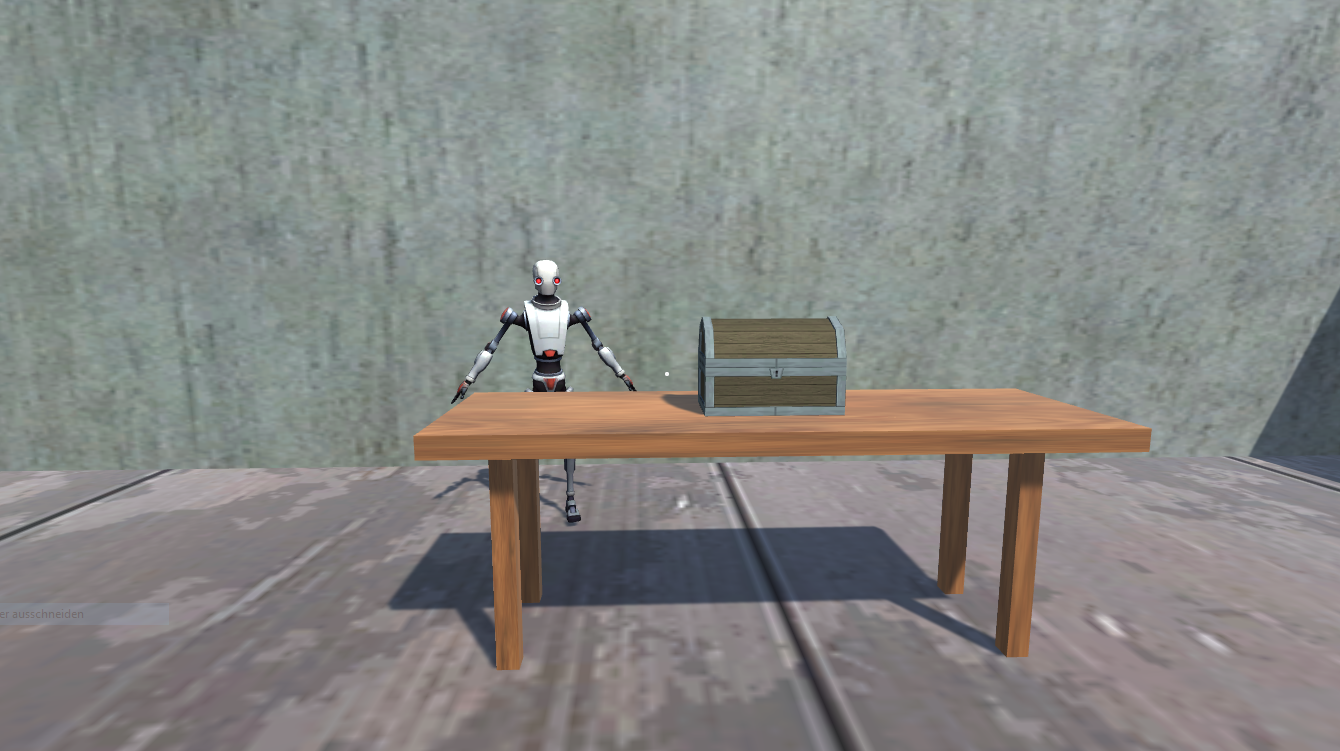
\includegraphics[width=0.75\textwidth]{InteractivityPrototype.PNG}
\caption{Ein Avatar des Prototyps}
\end{figure}

Um mehreren Spielern gleichzeitigen Zugriff auf die Anwendung zu geben, wird das PUN-Plugin von Photon verwendet. Über C\# Skripte werden sowohl die Verbindung zu dem Photon-Server hergestellt, als auch eine Lobby und ein Raum erstellt. ~\parencite{InfoGamer2018}
Hierbei muss nun beachtet werden, dass der Avatar nicht mehr im Voraus in der Szene platziert sein darf. Der erste Spieler kann diesen zwar kontrollieren, aber der zweite Spieler überschreibt die Kontrolle über den Avatar sobald er beitritt. Um dieses Problem zu lösen, werden die Avatare der Spieler über ein Skript dynamisch der Szene hinzugefügt, sobald diese beitreten. Somit muss die Anzahl der Spieler nicht im Voraus festgelegt werden. Um das neue Problem zu lösen, dass sich während des Beitritts keine verfügbare Kamera in der Szene befindet, wird eine zweite Szene in Form eines Menüs verwendet. Jeder Spieler der beitreten möchte befindet sich solange in diesem Menü, bis in der Hauptszene ein Avatar fertig vorbereitet ist, und wird dann in diese weitergeleitet. \newline

Alle Objekte die mehrfach instanziiert werden und über das Netzwerk identifiziert werden sollen, erhielten eine sogenannte PhotonView-Komponente. Die Skripte die für die Bewegungen des Avatars und der Kamera zuständig sind, beziehen sich bei einer Mehrspieler-Anwendung auf die lokale PhotonView-Komponente, um zu verhindern dass sich alle Instanzen bewegen. Ohne diese Vorkehrung könnte ein Benutzer alle Avatare in der Anwendung steuern. \\

Um die Interaktionen der Spieler mit ihrer Umgebung über alle Instanzen zu synchronisieren, wurde ein Remote Procedure Call (RPC) verwendet. Diese RPCs erlauben es Methoden von anderen Objekten im Netzwerk aufzurufen. In diesem Fall wurde hiermit das Öffnen und Schließen der Kiste synchronisiert. Wenn ein Benutzer auf die Kiste klickt, wird die RPC Methode jeder Instanz des Objektes aufgerufen, welche den Zustand der Kiste von geschlossen zu geöffnet ändert, und anders herum. Dies bedeutet dass die Kisten bei allen Benutzern, inklusive der Eigenen, ihren Zustand ändern, sobald ein Benutzer mit seiner Kiste interagiert. Dies erzeugt den Eindruck dass sich alle Benutzer im selben Raum befinden und mit der gleichen Kiste interagieren. Eine Sperrung der Kiste, um Kollisionen in der Interaktion zu verhindern, war in diesem Fall nicht notwendig. Sollte ein Benutzer mit der Kiste interagieren, während die Animation noch nicht abgeschlossen ist, wird die Animation abgebrochen und aus der aktuellen Position in die andere Richtung fortgesetzt. Wenn also mit einer sich schließenden Kiste interagiert wird bevor diese komplett geschlossen ist, wird nahtlos die Öffnungs-Animation aus der aktuellen Position ausgeführt. \newline 
Eine Möglichkeit die Interaktion mit Objekten zu erleichtern, ist eine Highlight-Funktion, welche in diesem Prototypen getestet wurde. Wenn ein Benutzer mit dem Cursor auf ein Objekt zielt mit dem interagiert werden kann, wird dieses farblich gekennzeichnet. Dies erleichtert es dem Benutzer zwischen dekorativen und interaktiven Objekten zu unterscheiden.

\subsection{ViRGOS}
In diesem Unterkapitel wird die Umsetzung der Funktionalitäten in ViRGOS thematisiert. Zu Beginn wird geschildert wie die Anwendung erweitert wurde, sodass diese mehrere Spieler gleichzeitig zulässt. Anschließend wird erklärt wie der Versuchsaufbau implementiert wurde, der für den Astronauten gedacht ist. Zum Abschluss wird auf die Werkzeuge eingegangen die für die Kommunikation zwischen den Benutzern zuständig sind. 

\subsubsection{Mehrspielerfähigkeit}
Um ViRGOS mit mehreren Spielern zu benutzen, wurden dieselben Schritte durchgeführt, die zuvor in Kapitel \ref{Vorstudie} getestet wurden. Nachdem das Photon-Plugin in das Projekt eingebunden war, wurden Skripte erstellt die einen Raum und eine Lobby erzeugen. Auch hier wurde der Avatar aus der Szene entfernt, um ihn dynamisch zu instanziieren sobald ein Benutzer beitritt. Zusätzlich zu der PhotonView, die für die Referenzierung über das Netzwerk notwendig ist, wurde der Avatar mit einer Photon Transform View ausgestattet, die die Position und die Rotation der Avatare über alle Instanzen der Anwendung synchronisiert.

\begin{figure}[H]
\centering
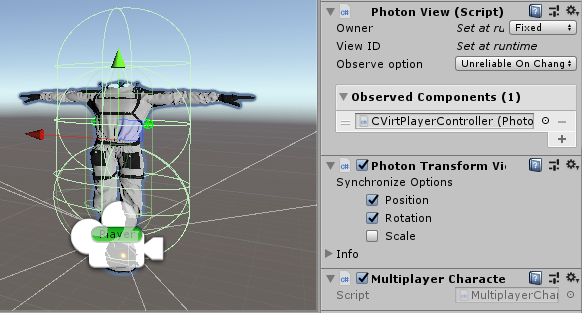
\includegraphics[width=0.75\textwidth]{UnityComponents.PNG}
\caption{Der Avatar mit Photons Multiplayer-Komponenten}
\end{figure}

Ebenso wurde eine Menü-Szene erstellt, die der Haupt-Szene Zeit gibt eine Instanz des Avatars zu erschaffen. Wie in dem Prototyp musste auch hier darauf geachtet werden, dass der Spieler nur seinen eigenen Avatar kontrollieren kann. Wenn ein Spieler beitritt, wird geprüft ob ein Avatar eine lokale Instanz ist oder nicht. Dies wird über die PhotonView Komponente erreicht. Wenn ein Avatar eine lokale Instanz ist, wird dieser von dem Benutzer gesteuert, der sich an dem Gerät befindet. Die Skripte die für die Bewegung des Avatars zuständig sind, werden bei allen Instanzen deaktiviert die nicht lokal sind. Somit kann ein Benutzer nur seinen eigenen Avatar kontrollieren.\\

Um die bereits existierenden Funktionen der Rakete und Aufzüge über das Netzwerk zu synchronisieren, wurden diese so angepasst, dass sie zentralisiert verarbeitet werden. Alle Funktionen der Rakete werden von einem zentralen Skript entgegengenommen. Auch die Funktionen der Aufzüge werden zentralisiert abgearbeitet. In diesen zentralen Skripten werden RPCs angewandt, um diese Aufrufe über die Instanzen zu synchronisieren. Betätigt ein Benutzer nun einen Knopf um beispielsweise eine Tür der Rakete zu öffnen, sendet das zentralisierte Skript einen RPC an alle Instanzen mit der Bezeichnung des betätigten Knopfes. Somit führen alle Instanzen die jeweilige Funktion aus die dem Knopf zugeordnet ist, was dazu führt, dass sich bei jedem Spieler die Tür der Rakete öffnet.

\begin{figure}[H]
\centering
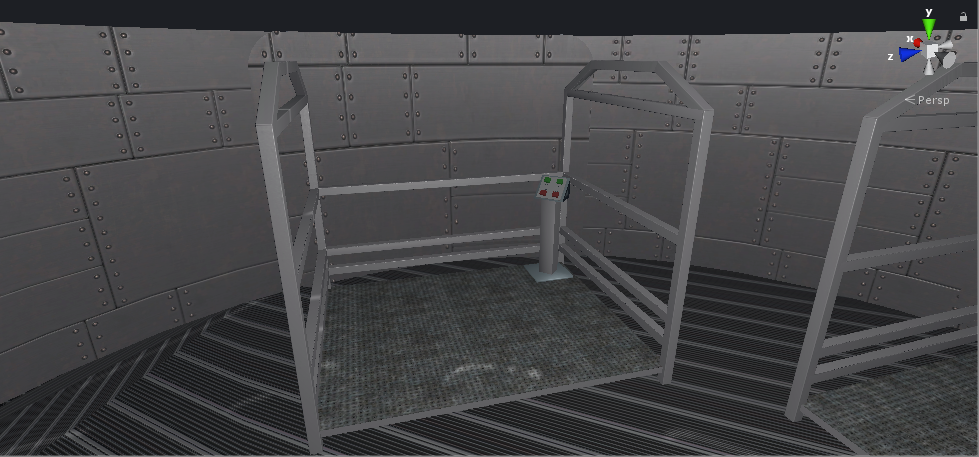
\includegraphics[width=0.75\textwidth]{Elevator.PNG}
\caption{Einer der Aufzüge mit dem zugehörigen Steuerpult}
\end{figure}

Um die Kollision von Interaktionen mehrerer Benutzer zu verhindern, wurde eine Stoppuhr in das Skript der zentralen Raketensteuerung implementiert. Diese Stoppuhr beginnt zu zählen, sobald ein Knopf in der Szene betätigt wird. Das zentrale Kontrollskript blockiert nun die Annahme von sämtlichen Signalen von Knöpfen für eine Sekunde. Dies verhindert, dass ein Knopf aus Versehen zu lange gedrückt wird, was von dem Programm als erneutes Drücken interpretiert werden kann. Außerdem wird so das Problem der Kollision von Interaktionen gelöst. Falls zwei Benutzer denselben Knopf zur gleichen Zeit drücken wollen, wird nur die erste Aktivierung angenommen, da der Knopf anschließend für eine Sekunde gesperrt ist.

\begin{figure}[H]
\centering
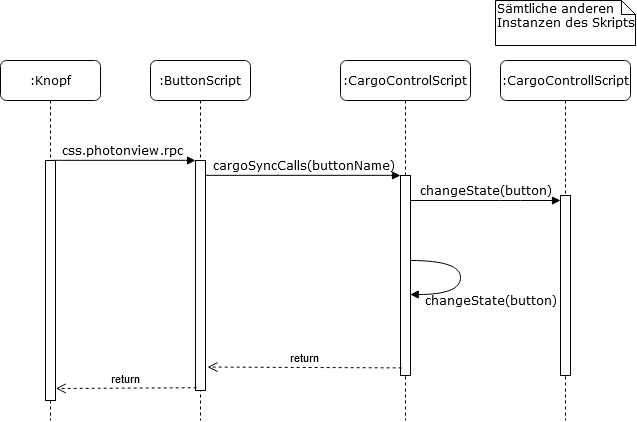
\includegraphics[width=1\textwidth]{RPC.PNG}
\caption{Sequenzdiagramm der RPCs}
\end{figure}

\subsubsection{Versuchsaufbau für Interaktionen}
Um die Interaktionen zwischen mehreren Benutzern testen zu können, musste zuerst eine Aufgabe entwickelt werden die die Benutzer lösen können. Da der Kommandant, wie im Kapitel \ref{Problemstellung} erklärt, den Astronauten anleiten soll, wurde sich für eine Problemstellung außerhalb der Rakete entschieden. Somit kann der Kommandant in dem Kontrollraum bleiben und den Astronauten unterstützen, während dieser einer Aufgabe nachgeht.

\begin{figure}[H]
\centering
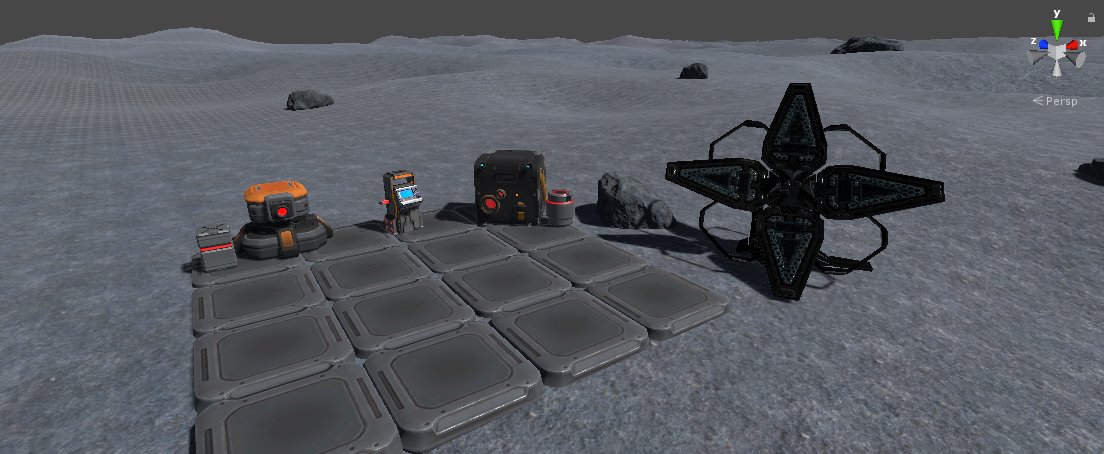
\includegraphics[width=1\textwidth]{InteraktionStation.PNG}
\caption{Der Versuchsaufbau außerhalb der Rakete}
\end{figure}

\subsubsection*{Erste Iteration}
In der ersten Iteration der interaktiven Aufgabe kamen Objekte aus dem Unity Asset Store zum Einsatz. Es wurde aus Gründen der Immersion darauf geachtet, dass diese zu der Weltraumthematik passen. Speziell ein futuristischer Geldautomat, ein Geschützturm, das Modell einer Drohne und eine Satellitenschüssel wurden ausgewählt, unter anderem weil diese kostenfrei verfügbar waren. 

\begin{figure}[H]
\centering
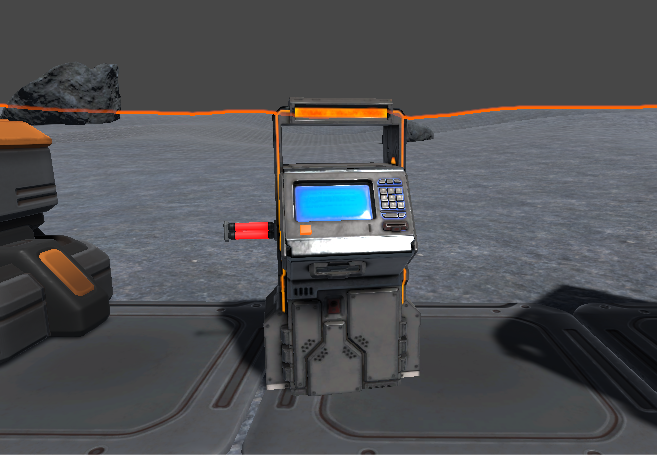
\includegraphics[width=0.8\textwidth]{ATM.PNG}
\caption{Das Modell des Geldautomaten}
\label{fig:ATM}
\end{figure}

Sowohl der Geschützturm, die Satellitenschüssel als auch der Geldautomat verfügen über keinerlei eigene Funktionen. Das Modell der Drohne verfügt über bewegliche Teile, die alle eigene Animationen besitzen. Zusätzlich wurde eine Sammlung von Fässern in verschiedenen Designs verwendet, einerseits um die Szene etwas mehr auszufüllen, andererseits um sie als Indikatoren zu verwenden. Jedes dieser Fässer besitzt eine leuchtende, farbige Komponente. Indem die Größe und Position der Fässer angepasst wird, können diese von den Spielern als Signallampe der interaktiven Objekte wahrgenommen werden. In Abbildung \ref{fig:ATM} ist das Modell des Geldautomaten zu sehen. An der linken Seite des Modells, befindet sich ein kleines, rotes Objekt. Dieses Objekt ist eines der Fässer, welches in diesem Fall als Indikator eingesetzt wird. 

\begin{figure}[H]
\centering
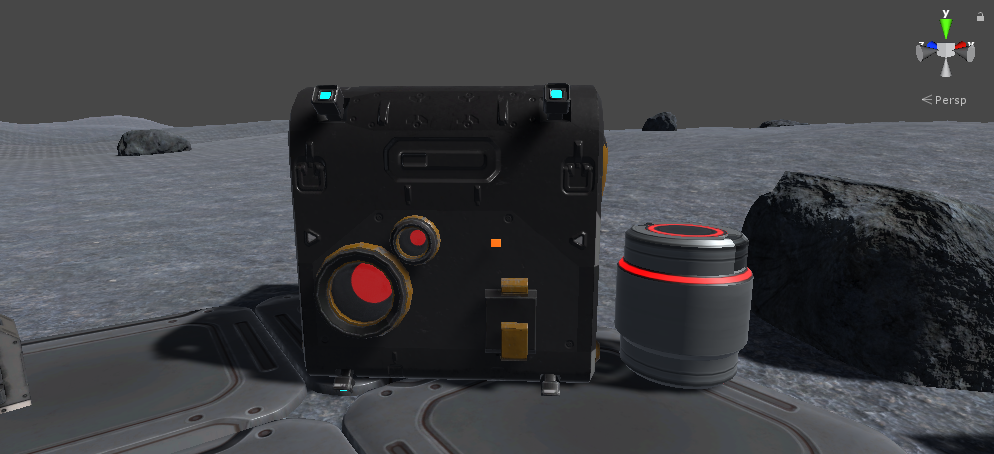
\includegraphics[width=0.8\textwidth]{Drone.PNG}
\caption{Das Modell der Drohne}
\end{figure}

Jede der interaktiven Maschinen wurde mit einem Knopf ausgestattet, der die Farbe der Fässer in unmittelbarer Nähe zwischen rot und grün wechselt. Dies soll den Eindruck erwecken, dass die Maschine an- oder ausgeschaltet ist. Das Modell der Drohne spielt zusätzlich die Animationen aller Einzelteile ab. Wenn alle Maschinen gleichzeitig angeschaltet sind, wechselt die Satellitenschüssel ihre Farbe von schwarz zu grün. Damit ist die Aufgabe für den Spieler abgeschlossen.\newline

\begin{figure}[H]
\centering
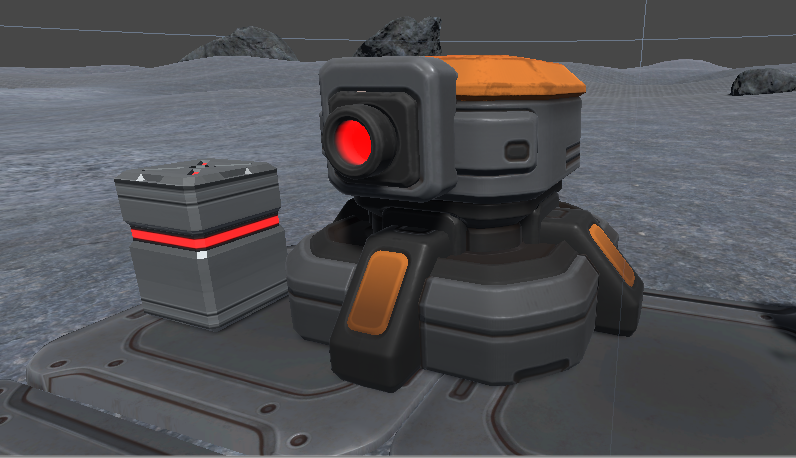
\includegraphics[width=0.8\textwidth]{Turret.PNG}
\caption{Das Modell des Geschützes}
\end{figure}

\begin{figure}[H]
\centering
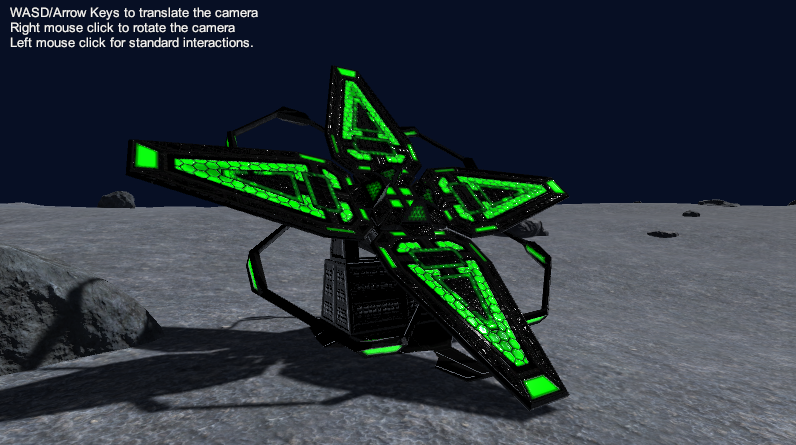
\includegraphics[width=0.8\textwidth]{SatelliteDish.PNG}
\caption{Die Satellitenschüssel in angeschaltetem Zustand}
\end{figure}

\subsubsection*{Zweite Iteration}
Um die Wahrscheinlichkeit zu erhöhen, dass der Astronaut Unterstützung bei der Lösung der Aufgabe benötigt, wurde der Versuchsaufbau weiterentwickelt. Die einzelnen Bauteile der Drohne verfügen bereits von Haus aus über Animationen, die die Objekte allerdings automatisch in die Ausgangsposition zurück bewegen. 

\begin{figure}[H]
\centering
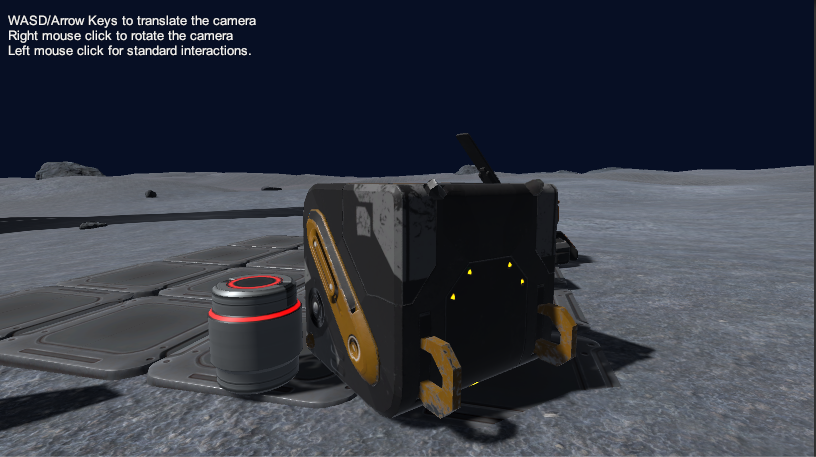
\includegraphics[width=0.8\textwidth]{DrohneGeschlossen.PNG}
\caption{Die Rückseite der Drohne in geschlossenem Zustand}
\end{figure}

Um dies zu verhindern wurden alle Animationen auf die Hälfte gekürzt. Die Einzelteile der Drohne bleiben somit in ihrer ausgefahrenen Position stehen, wodurch die Benutzer Zugriff auf den Innenraum der Drohne erhalten. Ein weiterer Druck auf den Knopf spielt die Animation nun rückwärts ab, und alle Einzelteile bewegen sich in ihre Ausgangsposition. Dies ermöglicht eine komplexere Aufgabenstellung, indem weitere Knöpfe im Inneren des Geräts versteckt wurden. Um die Drohne zu aktivieren, muss der Astronaut die Drohne öffnen, alle drei Knöpfe im Inneren aktivieren und diese wieder schließen.

\begin{figure}[H]
\centering
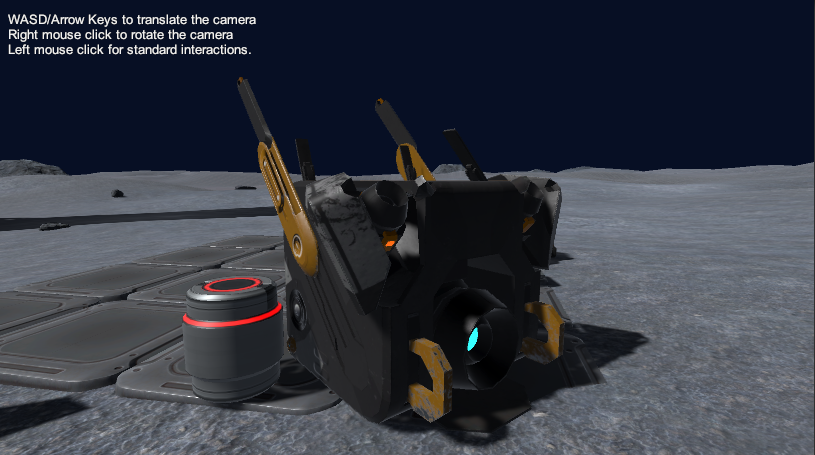
\includegraphics[width=0.8\textwidth]{DrohneOffen.PNG}
\caption{Die Rückseite der Drohne in geöffnetem Zustand}
\end{figure}

\subsubsection{Werkzeuge}
Damit der Kommandant den Astronauten anleiten kann, muss dieser wissen woran der Astronaut aktuell arbeitet. Da sich der Astronaut außerhalb der Rakete befindet, hat der Kommandant keinen direkten Blickkontakt zu ihm. ViRGOS war zu Beginn dieser Arbeit bereits mit einer Voice-Chat Funktion ausgestattet, was die Kommunikation ermöglicht. Die Anwendung wurde durch eine visuelle Komponente erweitert, die es dem Kommandanten ermöglicht zu sehen was der Astronaut gerade sieht. Hierfür wurde einer der drei Bildschirme des Kontrollraums verwendet. Dieser wurde mit einer Render-Textur ausgestattet. Hierbei handelt es sich um eine Textur mit der die Oberfläche eines Objektes definiert werden kann. Die Besonderheit ist, dass man diese Textur einer Kamera in der Szene zuweisen kann, die ihren aktuellen Sichtbereich auf die Textur rendert. Somit wird auf dem Objekt, das über die Textur verfügt, alles dargestellt was sich im Sichtbereich der Kamera befindet. Hierbei gibt es das Problem, dass eine Kamera immer nur ein Ziel für seine Darstellung haben kann. Dies bedeutet dass die Kamera entweder auf die Textur oder den Bildschirm des Benutzers rendern kann, aber nicht beides gleichzeitig. Um dies zu verhindern, wurde der Avatar des Benutzers mit einer zweiten Kamera ausgestattet, die speziell hierfür zum Einsatz kommt. Die Kamera ist standardmäßig deaktiviert und der Bildschirm somit ausgeschaltet. Die Schalttafel der Rakete wurde um weitere Knöpfe erweitert. Der erste Knopf aktiviert den Bildschirm, welcher die Sicht der Spieler darstellt. Dies geschieht über ein Skript, welches eine Liste aller aktuell aktiven Benutzer anlegt, welche dann nach ihrer ID sortiert werden. Somit wird sichergestellt dass alle Instanzen der Anwendung über die selbe Liste verfügen. Ohne diese Sortierung würde jede Instanz der Anwendung über eine unterschiedliche Liste der Spieler verfügen, da der lokale Avatar immer an erster Stelle steht. Anschließend wird die sekundäre Kamera des ersten Benutzers in der Liste aktiviert, welche nun ihre Sicht auf den Bildschirm rendert. Somit wird bei allen Benutzern der Anwendung, das Sichtfeld der selben Kamera auf den Bildschirm ausgegeben. Ein weiterer Druck auf den Knopf deaktiviert die aktuell aktive sekundäre Kamera und aktiviert die sekundäre Kamera des nächsten Benutzers in der Liste. Somit wird durch alle Benutzer iteriert, bis das Ende der Liste erreicht ist. Durch erneutes Betätigen des Knopfes wird der Bildschirm wieder ausgeschaltet und der Index des Iterators zurückgesetzt, was ein neues Durchlaufen der Liste ermöglicht. Diese Funktionalität erlaubt dem Kommandanten eine schnelle Lokalisierung des Astronauten, aber auch von allen anderen Benutzern. Durch die Positionierung und die Entfernungen des Bildschirms zu den Benutzern ist es allerdings schwer, potentiell wichtige Details zu erkennen.\newline

\begin{figure}[H]
\centering
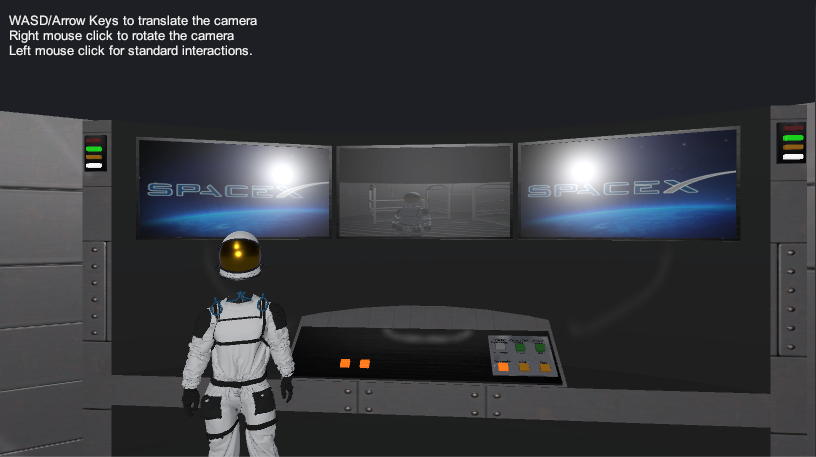
\includegraphics[width=0.8\textwidth]{VirgosScreenview.PNG}
\caption{Einer der Avatare, während seine Sicht auf dem Bildschirm dargestellt wird}
\end{figure}

Eine Erweiterung der Funktion ist das Wechseln der primären Kamera auf die sekundäre Kamera des jeweiligen Benutzers. Dies ermöglicht es dem Kommandanten durch die Augen des Astronauten zu sehen und so genauere Anweisungen zu geben oder mögliche Probleme zu identifizieren die nicht über den Voice-Chat kommuniziert werden können. Durch einen Druck auf den zweiten Knopf kann die lokale primäre Kamera mit der sekundären Kamera getauscht werden, die aktuell auf dem Bildschirm angezeigt wird. Dies geschieht indem die primäre Kamera und gleichzeitig die Render-Textur der sekundären Kamera des jeweiligen Avatars deaktiviert werden. Somit wird das Bild der sekundären Kamera nicht mehr auf dem Bildschirm in der Anwendung angezeigt, sondern auf dem echten Bildschirm des Benutzers. 

\begin{figure}[H]
\centering
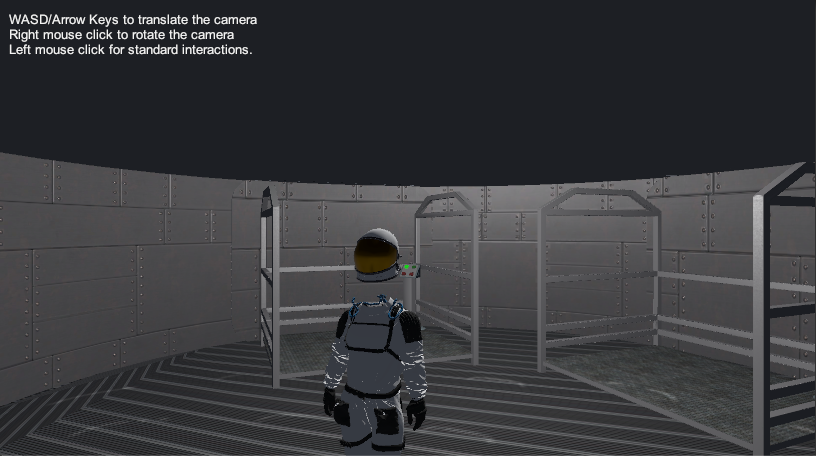
\includegraphics[width=0.8\textwidth]{ScreenDuplicate.PNG}
\caption{Die Sicht des Avatars, während sie den kompletten Bildschirm ausfüllt}
\end{figure}

\subsection{Einschränkungen durch Covid-19}
Aufgrund der Covid-19-Pandemie und den daraus resultierenden Kontaktverboten und Schließungen von öffentlichen Einrichtungen, wirkte sich dies auch auf die Entwicklung dieses Projektes aus. Da sich das einzige verfügbare Virtual Reality Headset im Labor der Hochschule Reutlingen befand, erschwerte dies das Testen der Anwendung. Viele Funktionen konnten ohne Headset an einem Computer getestet werden, für Andere war das Testen mit einem Headset aber unumgänglich. Hierfür wurde mit einem Kommilitonen der Hochschule zusammengearbeitet, der privat über ein Headset verfügt. Dieser war freundlicherweise bereit die Anwendung in Virtual Reality zu testen und Besonderheiten oder Fehler über einen Voice-Chat zu schildern. Somit konnte zumindest regelmäßig auf Fehler reagiert, und diese behoben werden. \newline
Auch die Probandenbefragung war in der geplanten Form nicht durchführbar, da diese Aufgrund der benötigten Hardware nur in der Hochschule umsetzbar gewesen wäre. 